\documentclass[11pt, a4paper, leqno]{article}
\usepackage{a4wide}
\usepackage[T1]{fontenc}
\usepackage[utf8]{inputenc}
\usepackage{float, afterpage, rotating, graphicx}
\usepackage{epstopdf}
\usepackage{longtable, booktabs, tabularx}
\usepackage{fancyvrb, moreverb, relsize}
\usepackage{eurosym, calc, chngcntr}
\usepackage{amsmath, amssymb, amsfonts, amsthm, bm}
\usepackage{caption}
\usepackage{mdwlist}
\usepackage{xfrac}
\usepackage{setspace}
\usepackage{xcolor}
% \usepackage{pdf14} % Enable for Manuscriptcentral -- can't handle pdf 1.5
% \usepackage{endfloat} % Enable to move tables / figures to the end. Useful for some submissions.

\usepackage[
    natbib=true,
    bibencoding=inputenc,
    bibstyle=authoryear-ibid,
    citestyle=authoryear-comp,
    maxcitenames=3,
    maxbibnames=10,
    useprefix=false,
    sortcites=true,
    backend=biber
]{biblatex}
\AtBeginDocument{\toggletrue{blx@useprefix}}
\AtBeginBibliography{\togglefalse{blx@useprefix}}
\setlength{\bibitemsep}{1.5ex}
\addbibresource{refs.bib}

\usepackage[unicode=true]{hyperref}
\hypersetup{
    colorlinks=true,
    linkcolor=black,
    anchorcolor=black,
    citecolor=black,
    filecolor=black,
    menucolor=black,
    runcolor=black,
    urlcolor=black
}


\widowpenalty=10000
\clubpenalty=10000

\setlength{\parskip}{1ex}
\setlength{\parindent}{0ex}
\setstretch{1.5}


\begin{document}

\title{TTT
\thanks{NNN: UUU, Address. \href{mailto:x@y.z} {\nolinkurl{x [at] y [dot] z}}, tel.~+00000.}
% subtitle: 
% \\[1ex] 
% \large Subtitle here
}

\author{NNN
% \\[1ex]
% Additional authors here
}

\date{
{\bf Preliminary -- please do not quote} 
\\[1ex] 
\today
}

\maketitle


\begin{abstract}
	Some abstract here.
\end{abstract}
\clearpage

\section{Introduction} % (fold)
\label{sec:introduction}

If you are using this template, please cite this item from the references: \citet{GaudeckerEconProjectTemplates}

Some text here. Example for a formula inclusion:

\input{formulas/some_formula}

\begin{table}[h!]
    \caption{Demonstrating inclusion of files}
    \label{tab:demonstrating_inclusion_of_files}
    \begin{center}
        % This is just a dummy table.
\begin{tabular}{rr}
    \toprule
    Nothing & Something \tabularnewline 
    \midrule
    0       & 1.1       \tabularnewline
    0       & 4.5       \tabularnewline 
    \bottomrule
\end{tabular}

    \end{center}
    \footnotesize
    \emph{Note:} One could also define commands in {\LaTeX} for the paths to the graphics and tables directories. I prefer not to do so since the Waf scanner won't find them automatically (I believe), but in the end it's a matter of taste where you want to do manual work (i.e. in the {\LaTeX} files or in the wscript files).
\end{table}


Some text here. Example for a formula inclusion:

\begin{figure}
    \caption{Segregation by cycle in the baseline \citet{Schelling69} model as in the \citet{StachurskiSargent13} example}
    
    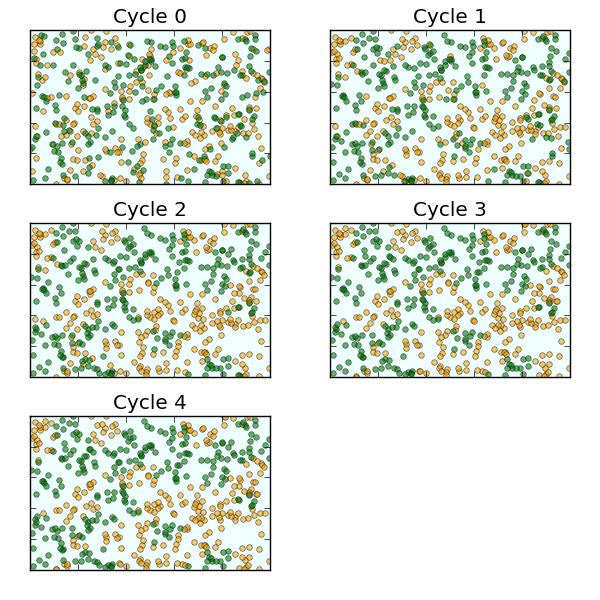
\includegraphics[width=\textwidth]{../../out/figures/schelling_baseline}

\end{figure}

\begin{figure}
    \caption{Segregation by cycle in the baseline \citet{Schelling69} model, limiting the number of potential moves per period to two}
    
    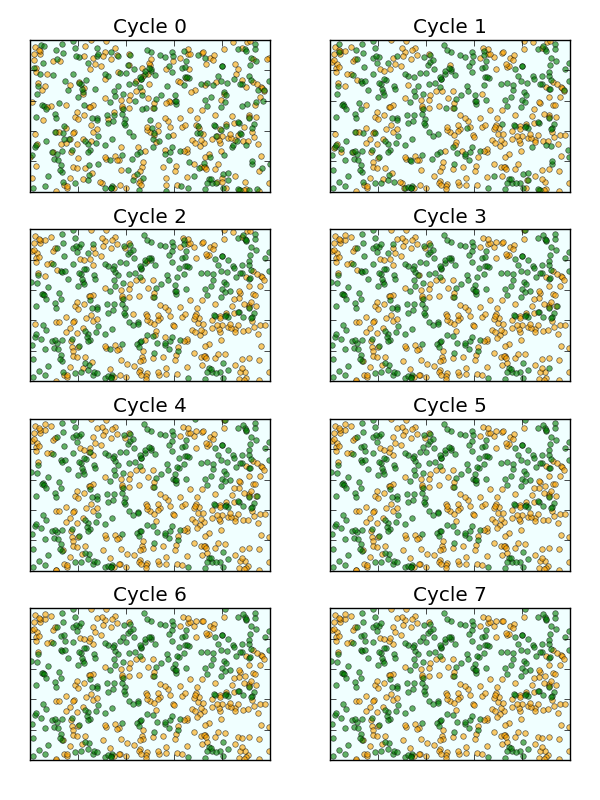
\includegraphics[width=\textwidth]{../../out/figures/schelling_max_moves_2}

\end{figure}


% section introduction (end)



\setstretch{1}
\printbibliography
\setstretch{1.5}

%\appendix
%\counterwithin{table}{section}
%\counterwithin{figure}{section}

\end{document}
